%!TEX root = ../thesis.tex
% chktex-file 1
% chktex-file 2
% chktex-file 24
% ******************************* Thesis Appendix A ****************************
\chapter{Latches small signal models}
\label{appx:latch_models}
%**************** Comparator Small Signal Model and Equations *******************
\section{Strong Arm}
In order to derive offset and delay equations, the small signal model of the strong arm latch is represented in \figurename~\ref{fig:annexe_sa_small_signal}. The drain-source effect of transistors is neglected for the sake of simplicity. These are considered then in the post-layout simulation results presented in Section~\ref{sec:latches_sim}

\begin{figure}[htp]
\centering
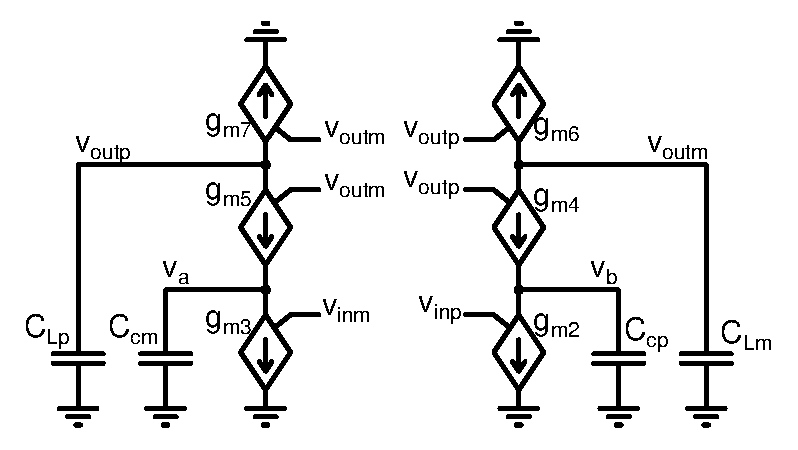
\includegraphics[width=\textwidth]{Chapter7/Figs/sa_small_signal_model.ps}
\caption{Strong Arm Small Signal Model}
\label{fig:annexe_sa_small_signal}
\end{figure}

The application of KCL at nodes \(v_a\) and \(v_b\) gives respectively
\begin{align}
    \left(sC_{cm}+g_{m5}\right)v_a &= g_{m5}v_{outm} - g_{m3}v_{inm} \\
    \left(sC_{cp}+g_{m4}\right)v_b &= g_{m4}v_{outp} - g_{m2}v_{inp}
    \label{eqn:annexe_va_vb}
\end{align}

while KCL on output nodes lead to
\begin{align}
    sC_{Lp} v_{outp} &= -(g_{m5}+g_{m7})v_{outm} + g_{m5}v_{a} \\
    sC_{Lm} v_{outm} &= -(g_{m4}+g_{m6})v_{outp} + g_{m4}v_{b}
\end{align}

Replacing \(v_{a} \) and \(v_{b} \) in these equation by their expression in~\ref{eqn:annexe_va_vb} gives us
\begin{align}
    sC_{Lp} v_{outp} &= -(g_{m5}+g_{m7})v_{outm} + \frac{g_{m5}}{1+s\frac{C_{cm}}{g_{m5}}}v_{outm} - \frac{g_{m3}}{1+s\frac{C_{cm}}{g_{m5}}}v_{inm} \\
    sC_{Lm} v_{outm} &= -(g_{m4}+g_{m6})v_{outp} + \frac{g_{m4}}{1+s\frac{C_{cp}}{g_{m4}}}v_{outp} - \frac{g_{m2}}{1+s\frac{C_{cp}}{g_{m4}}}v_{inp}
\end{align}

Then, voltages are defined in term of their common mode voltage and differential voltages such that \(v_{inp} = v_{inc}+v_{ind}/2\) and \(v_{inm} = v_{inc}-v_{ind}/2\) (resp.\ for \(v_{outp}\) and \(v_{outm}\)).

\begin{align}
    s\left(C_{Lp}-C_{Lm}\right) v_{outc} + s\left(C_{Lp}+C_{Lm}\right) \frac{v_{outd}}{2} &= (g_{m4}+g_{m6}-g_{m5}-g_{m7}) v_{outc} \\
    &+ (g_{m4}+g_{m6}+g_{m5}+g_{m7}) v_{outd} \nonumber \\
    &+ v_{outc} \left(\frac{g_{m5}}{1+s\frac{C_{cm}}{g_{m5}}} - \frac{g_{m4}}{1+s\frac{C_{cp}}{g_{m4}}}\right) \nonumber \\
    &- \frac{v_{outd}}{2} \left(\frac{g_{m5}}{1+s\frac{C_{cm}}{g_{m5}}} + \frac{g_{m4}}{1+s\frac{C_{cp}}{g_{m4}}}\right) \nonumber \\
    &+ v_{inc} \left(\frac{g_{m3}}{1+s\frac{C_{cm}}{g_{m5}}} - \frac{g_{m2}}{1+s\frac{C_{cp}}{g_{m4}}}\right) \nonumber \\
    &- \frac{v_{ind}}{2} \left(\frac{g_{m3}}{1+s\frac{C_{cm}}{g_{m5}}} + \frac{g_{m2}}{1+s\frac{C_{cp}}{g_{m4}}}\right) \nonumber
\end{align}

The input referred offset could be defined as the differential input voltage when the differential output voltage is null, the offset is thus defined as

\begin{align}
    \frac{v_{offset}}{2} \left( \frac{g_{m3}}{1+s\frac{C_{cm}}{g_{m5}}} + \frac{g_{m2}}{1+s\frac{C_{cp}}{g_{m4}}} \right) &= \left( g_{m4}+g_{m6}-g_{m5}-g_{m7}-s\left(C_{Lp}-C_{Lm}\right) \right) v_{outc} \\
    &+ v_{outc} \left( \frac{g_{m5}}{1+s\frac{C_{cm}}{g_{m5}}} - \frac{g_{m4}}{1+s\frac{C_{cp}}{g_{m4}}} \right) \nonumber \\
    &+ v_{inc} \left( \frac{g_{m3}}{1+s\frac{C_{cm}}{g_{m5}}} - \frac{g_{m2}}{1+s\frac{C_{cp}}{g_{m4}}} \right) \nonumber
\end{align}

\section{Strong Arm Montanaro Version}
The transistor introduced by Montanaro in~\cite{Montanaro1996} keep a the voltage defined at drain of differential pair transistors even if the differential input is extremely large.
Unfortunately, this extra ``resistor'' implemented by a mosfet alter the decision in both the offset and the delay required to make a decision.

The small signal model is represented in 

\begin{figure}[htp]
    \centering
    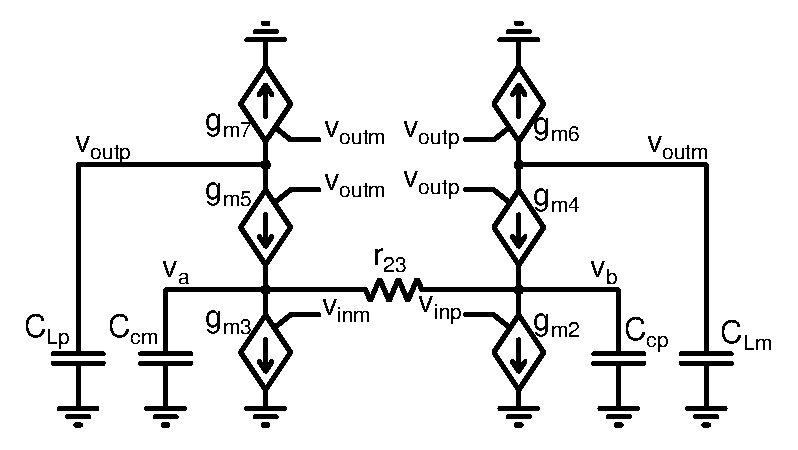
\includegraphics[width=\textwidth]{Chapter7/Figs/sa_montanaro_small_signal_model.ps}
    \caption{Strong Arm Small Signal Model}
    \label{fig:annexe_sa_montanaro_small_signal}
\end{figure}

Compared to conventional structure, KCL on output nodes lead to the same equations which are
\begin{align}
    sC_{Lp} v_{outp} &= -(g_{m5}+g_{m7})v_{outm} + g_{m5}v_{a} \\
    sC_{Lm} v_{outm} &= -(g_{m4}+g_{m6})v_{outp} + g_{m4}v_{b}
\end{align}

while KCL applied on nodes \(v_a\) and \(v_b\) gives respectively
\begin{align}
    \label{eqn:annexe_va_vb_montanaro}
    \left(sC_{cm}+g_{m5}\right)v_a &= \frac{v_{b}-v_{a}}{r_{23}} + g_{m5}v_{outm} - g_{m3}v_{inm} \\
    \left(sC_{cp}+g_{m4}\right)v_b &= \frac{v_{a}-v_{b}}{r_{23}} + g_{m4}v_{outp} - g_{m2}v_{inp}
\end{align}

From each of these, \[
\begin{cases}
    \frac{v_a}{r_{23}} = \frac{v_{b}}{r_{23}^2\left(sC_{cm}+g_{m5}+\frac{1}{r_{23}}\right)} + \frac{g_{m5}v_{outm} - g_{m3}v_{inm}}{r_{23}\left(sC_{cm}+g_{m5}+\frac{1}{r_{23}}\right)} \\
    \frac{v_b}{r_{23}} = \frac{v_{a}}{r_{23}^2\left(sC_{cp}+g_{m4}+\frac{1}{r_{23}}\right)} + \frac{g_{m4}v_{outp} - g_{m2}v_{inp}}{r_{23}\left(sC_{cp}+g_{m4}+\frac{1}{r_{23}}\right)}
\end{cases}
\]
which put in one the other gives us \[
\begin{cases}
    \left(sC_{cm}+g_{m5}+\frac{1}{r_{23}}\right)v_a = \frac{v_{a}}{r_{23}^2\left(sC_{cp}+g_{m4}+\frac{1}{r_{23}}\right)} + \frac{g_{m4}v_{outp} - g_{m2}v_{inp}}{r_{23}\left(sC_{cp}+g_{m4}+\frac{1}{r_{23}}\right)} + g_{m5}v_{outm} - g_{m3}v_{inm}  \\
    \left(sC_{cp}+g_{m4}+\frac{1}{r_{23}}\right)v_b = \frac{v_{b}}{r_{23}^2\left(sC_{cm}+g_{m5}+\frac{1}{r_{23}}\right)} + \frac{g_{m5}v_{outm} - g_{m3}v_{inm}}{r_{23}\left(sC_{cm}+g_{m5}+\frac{1}{r_{23}}\right)} + g_{m4}v_{outp} - g_{m2}v_{inp}
\end{cases}
\]

This simplifies as \[
\begin{cases}
v_a = \frac{r_{23}\left(g_{m4}v_{outp}-g_{m2}v_{inp}\right)+r_{23}^2\left(g_{m5}v_{outm}-g_{m3}v_{inm}\right)\left(sC_{cp}+g_{m4}+\frac{1}{r_{23}}\right)}{r_{23}^2\left(sC_{cp}+g_{m4}+\frac{1}{r_{23}}\right)\left(sC_{cm}+g_{m5}+\frac{1}{r_{23}}\right)-1} \\
v_b = \frac{r_{23}\left(g_{m5}v_{outm}-g_{m3}v_{inm}\right)+r_{23}^2\left(g_{m4}v_{outp}-g_{m2}v_{inp}\right)\left(sC_{cm}+g_{m5}+\frac{1}{r_{23}}\right)}{r_{23}^2\left(sC_{cp}+g_{m4}+\frac{1}{r_{23}}\right)\left(sC_{cm}+g_{m5}+\frac{1}{r_{23}}\right)-1}
\end{cases}
\]

We can already notice that for large \(r_{23}\) this acts much alike to the conventional circuit. While for small value of the resistance, the variation of \(v_a\) and \(v_b\) are slowed down.

Expressed as a function of the common and the differential component, this trends is clearer where \(\gamma = r_{23}^2\left(sC_{cp}+g_{m4}+\frac{1}{r_{23}}\right)\left(sC_{cm}+g_{m5}+\frac{1}{r_{23}}\right)-1\):

\[
\begin{cases}
v_a &= \frac{g_{m4}r_{23}+g_{m5}r_{23}^2\left(sC_{cp}+g_{m4}+\frac{1}{r_{23}}\right)}{\gamma} v_{outc} - \frac{g_{m2}r_{23}+g_{m3}r_{23}^2\left(sC_{cp}+g_{m4}+\frac{1}{r_{23}}\right)}{\gamma} v_{inc} \\
&+ \frac{g_{m4}r_{23}-g_{m5}r_{23}^2\left(sC_{cp}+g_{m4}+\frac{1}{r_{23}}\right)}{\gamma} \frac{v_{outd}}{2} + \frac{-g_{m2}r_{23}+g_{m3}r_{23}^2\left(sC_{cp}+g_{m4}+\frac{1}{r_{23}}\right)}{\gamma} \frac{v_{ind}}{2} \\
v_b &= \frac{g_{m5}r_{23}+g_{m4}r_{23}^2\left(sC_{cm}+g_{m5}+\frac{1}{r_{23}}\right)}{\gamma} v_{outc} - \frac{g_{m3}r_{23}+g_{m2}r_{23}^2\left(sC_{cm}+g_{m5}+\frac{1}{r_{23}}\right)}{\gamma} v_{inc} \\
&+ \frac{-g_{m5}r_{23}+g_{m4}r_{23}^2\left(sC_{cm}+g_{m5}+\frac{1}{r_{23}}\right)}{\gamma} \frac{v_{outd}}{2} + \frac{g_{m3}r_{23}-g_{m2}r_{23}^2\left(sC_{cm}+g_{m5}+\frac{1}{r_{23}}\right)}{\gamma} \frac{v_{ind}}{2}
\end{cases}
\]

Finally, the offset can be found by setting \(v_{outd} = 0\) which gives us 
\small
\begin{align}
    \frac{v_{offset}}{2} & \left(g_{m5}g_{m3}r_{23}^2\left(sC_{cp}+g_{m4}+\frac{1}{r_{23}}\right)+g_{m4}g_{m2}r_{23}^2\left(sC_{cm}+g_{m5}+\frac{1}{r_{23}}\right)-r_{23}\left(g_{m4}g_{m3}+g_{m5}g_{m2} \right) \right) \\
 &= \left(s\left(C_{Lp}-C_{Lm}\right)+g_{m7}+g_{m5}-g_{m6}-g_{m4}\right) v_{outc}\gamma \nonumber \\
 &- \left(g_{m5}^2\left(sC_{cp}+g_{m4}+\frac{1}{r_{23}}\right)-g_{m4}^2\left(sC_{cm}+g_{m5}+\frac{1}{r_{23}}\right)\right) v_{outc}r_{23}^2  \nonumber \\
 &- \left(g_{m4}g_{m2}r_{23}^2\left(sC_{cm}+g_{m5}+\frac{1}{r_{23}}\right)-g_{m5}g_{m3}r_{23}^2\left(sC_{cp}+g_{m4}+\frac{1}{r_{23}}\right)+r_{23}\left(g_{m4}g_{m3}-g_{m5}g_{m2}\right) \right) v_{inc} \nonumber
\end{align}
\normalsize

Despite the extra complexity this engender, the static offset (for s=0) is greater than the static offset of the traditional version for large \(r_{23}\). Indeed, the \(\gamma\) factor acts share the same equation than a cascode. This boosting the mismatch error with the output common mode voltage. Others errors are also boosted if \small \[ \left(g_{m5}g_{m3}r_{23}^2\left(sC_{cp}+g_{m4}+\frac{1}{r_{23}}\right)+g_{m4}g_{m2}r_{23}^2\left(sC_{cm}+g_{m5}+\frac{1}{r_{23}}\right)-r_{23}\left(g_{m4}g_{m3}+g_{m5}g_{m2} \right) \right) < g_{m2}+g_{m3}.\]
\normalsize

In term of delay, the differential output is expressed in function of the differential input as
\small
\begin{align}
    v_{outd} & \Biggl[ s \left( C_{Lp}+C_{Lm}\right) -(g_{m4}+g_{m5}+g_{m6}+g_{m7})+ \\
    & \frac{g_{m4}^2 r_{23}^2 \left( sC_{cm}+g_{m5}+\frac{1}{r_{23}} \right) +g_{m5}^2 r_{23}^2 \left( sC_{cp}+g_{m4}+\frac{1}{r_{23}} \right) - 2g_{m4}g_{m5}r_{23}}{\gamma} \Biggr] = \nonumber \\
    v_{ind} & \frac{g_{m5}g_{m3}r_{23}^2 \left( sC_{cp}+g_{m4}+\frac{1}{r_{23}} \right) +g_{m4}g_{m2}r_{23}^2 \left( sC_{cm}+g_{m5}+\frac{1}{r_{23}} \right) -g_{m5}g_{m2}r_{23}-g_{m4}g_{m3}r_{23}}{\gamma} \nonumber
\end{align}
\normalsize

which decompose as a gain factor and a time constant for the generation: the time constant is given to be
\begin{align}
\tau &\approx \frac{\left(C_{Lp}+C_{Lm}\right)\gamma_0+g_{m4}^2r_{23}^2C_{cm}+g_{m5}^2r_{23}^2C_{cp}}{-(g_{m4}+g_{m5}+g_{m6}+g_{m7})\gamma_0+g_{m4}^2 r_{23}^2 \left(g_{m5}+\frac{1}{r_{23}} \right) +g_{m5}^2 r_{23}^2 \left(g_{m4}+\frac{1}{r_{23}} \right) - 2g_{m4}g_{m5}r_{23}}
\end{align}

The time constant expression is very similar to the one of the conventional strong arm. The part depending on \(r_{23}\) cannot be negative if the product of \(g_{m4}r_{23}\) and \(g_{m5}r_{23}\) are both greater than 1. \(\gamma_0 = \gamma(s=0) \) being strictly positive, the time constant is reduced.

An interesting observation is for a perfectly matching where \(g_{m}=g_{m4}=g_{m5}\), \(C_c=C_{cp}=C_{cm}\), and \(C_L=C_{Lp}=C_{Lm}\). The time constant reduces to
\[
    \tau \approx \frac{C_L\gamma_0+2g_{m}^2r_{23}^2C_c}{-(2g_{m}+g_{m6}+g_{m7})\gamma-0+g_{m}^2 r_{23}^2 \left(g_{m}+\frac{1}{r_{23}} \right) +g_{m}^2 r_{23}^2 \left(g_{m}+\frac{1}{r_{23}} \right) - 2g_{m}^2r_{23}}
\] 

for which the limit for large \(r_{23}\) gives
\[
    \lim_{r_{23}\to+\infty} \tau = \frac{C_L+2C_c}{-(2g_{m}+g_{m6}+g_{m7})+2g_{m}}
\]

In a way, even a very large resistance almost reach the same performance at the exception of parasitics introduced at nodes which increase \(C_c\) capacitance over the conventional circuit. Otherwise, extra \(g_{m}^2r_{23}\) in the denominator further reduce the time constant. In addition, the pmos transistors in the regeneration are those improving most the speed.

This indicates a trade-off between the delay and the offset for this architecture which is not the case of the version introduced in~\cite{Verbruggen2008}.

\section{Double Tail}
Similarly to the SA latch, this section presents the details for the offset calculus and the model used to derive the offset and the delay equation. The small signal model of the Schinkel version is represented in 

\begin{figure}[htp]
    \centering
    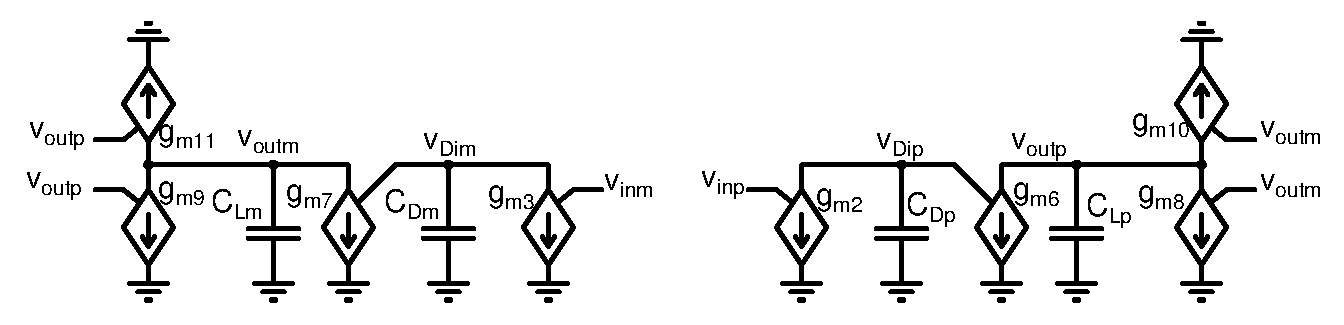
\includegraphics[width=\textwidth]{Chapter7/Figs/dtl_small_signal_model.ps}
    \caption{Double Tail Small Signal Model}
    \label{fig:annexe_dtl_schinkel_small_signal}
\end{figure}

The application of KCL on \(v_{Dix}\) nodes results in 
\[
\begin{cases}
    sC_{Dp}v_{Dip} = -g_{m2}v_{inp} \\
    sC_{Dm}v_{Dim} = -g_{m3}v_{inm} \\
\end{cases}
\]

while KCL on output nodes gives us
\[
\begin{cases}
    sC_{Lp}v_{outp} = -g_{m6}v_{Dip}-\left(g_{m8}+g_{m10}\right)v_{outm} \\
    sC_{Lm}v_{outm} = -g_{m7}v_{Dim}-\left(g_{m9}+g_{m11}\right)v_{outp} \\
\end{cases}
\]

Thus, the output voltages goes as
\begin{align}
\frac{v_{outd}}{2} \left(s\left(C_{Lp}+C_{Lm} \right)-g_{m8}-g_{m9}-g_{m10}-g_{m11} \right) &= 
-\frac{v_{ind}}{2} \left(\frac{g_{m6}g_{m2}}{sC_{Dp}}+\frac{g_{m7}g_{m3}}{sC_{Dm}} \right) \\
&+ v_{inc} \left(\frac{g_{m6}g_{m2}}{sC_{Dp}}-\frac{g_{m7}g_{m3}}{sC_{Dm}} \right) \nonumber \\
&+ v_{outc} \left(s\left(C_{Lp}-C_{Lm} \right)+g_{m8}+g_{m10}-g_{m9}-g_{m11} \right) \nonumber
\end{align}

Assuming \(v_{outd} = 0\) for the calculation of the input referred offset, the latter dependent on the input/output common mode and on mismatches as follow:

\begin{align}
\frac{v_{offset}}{2} \left(\frac{g_{m6}g_{m2}}{sC_{Dp}}+\frac{g_{m7}g_{m3}}{sC_{Dm}} \right) &= + v_{inc} \left(\frac{g_{m6}g_{m2}}{sC_{Dp}}-\frac{g_{m7}g_{m3}}{sC_{Dm}} \right) \\
&+ v_{outc} \left(s\left(C_{Lp}-C_{Lm} \right)+g_{m8}+g_{m10}-g_{m9}-g_{m11} \right) \nonumber
\end{align}
